\subsection{Requirements and Technology Baseline}
\subsubsection{Primo periodo  06/11/2023 - 24/11/2023}
    Nel corso del primo periodo, il nostro team ha dedicato risorse significative all'elaborazione e alla standardizzazione dei processi, formalizzando tali linee guida nel documento "Norme di Progetto". In quest'ultimo, sono state dettagliatamente redatte le sezioni specificate nella tabella sottostante.

    Durante il primo incontro con l'azienda, abbiamo definito obiettivi chiave da conseguire entro il prossimo SAL fissato per il 24 novembre 2023, coincidente con l'avvio del prossimo periodo. Questo approccio ricalca la struttura dello sprint backlog di Scrum.
    Tra i molteplici obiettivi delineati, si evidenziano la realizzazione di almeno un simulatore di un sensore in linguaggio Python, il quale interagisca con un server Kafka mediante Docker. Opzionalmente, si è prevista l'integrazione con il database ClickHouse per immagazzinare i dati dei simulatori. In parallelo, ci si è dedicati alla creazione di user story e casi d'uso correlati al capitolato.

    È soddisfacente constatare che tutte le richieste avanzate dal proponente sono state risolte entro i tempi concordati, includendo le richieste opzionali.

    Parallelamente, durante questa fase, gli amministratori hanno investito risorse per automatizzare il processo di compilazione dei sorgenti \LaTeX , una volta caricati nella repository condivisa. Inoltre, è stata implementata una procedura automatica di rinomina dei file PDF generati, inclusiva dell'indicazione della versione.

\paragraph{Rischi occorsi, impatto, mitigazione} 

Nel corso del primo periodo, si sono presentate le seguenti problematiche:
\begin{itemize}
    \item \textbf{Inesperienza nell'uso dell'ambiente Docker - \ref{sec:rischioTec}}
    \begin{itemize}
        \item \textbf{Esito mitigazione:} 
            L'autoapprendimento e la conoscenze dei singoli non si sono dimostrate adeguate per acquisire una conoscenza approfondita dell'ambiente Docker nel breve periodo iniziale, portando all'utilizzo del sistema senza una comprensione approfondita di ciascuna delle sue componenti e configurazioni. Di conseguenza, è stata formulata una richiesta al proponente per la realizzazione di un corso di formazione specifico su Docker seguendo le norme di mitigazione definite in \ref{sec:rischioTec}.
        \item \textbf{Impatto:}
            Nessuna conseguenza significativa è stata riscontrata, poiché le avvertenze segnalate dalla proponente riguardavano criticità di lieve entità relative alle best practices di Docker. Le misure di mitigazione necessarie sono state tempestivamente implementate, e un incontro formativo è stato programmato per approfondire ulteriormente la questione.
            Inoltre, al fine di conformarsi alle best practices dell'ambiente, è stata presa la decisione di regolamentare, nel documento "Norme di Progetto", lo sviluppo degli ambienti Docker.
    \end{itemize}
\end{itemize}

\newpage
\paragraph{Pianificazione attività divise per ruoli con consuntivo e preventivo orario e dei costi}\hspace{1pt}

\begin{figure}[H]
    \centering
    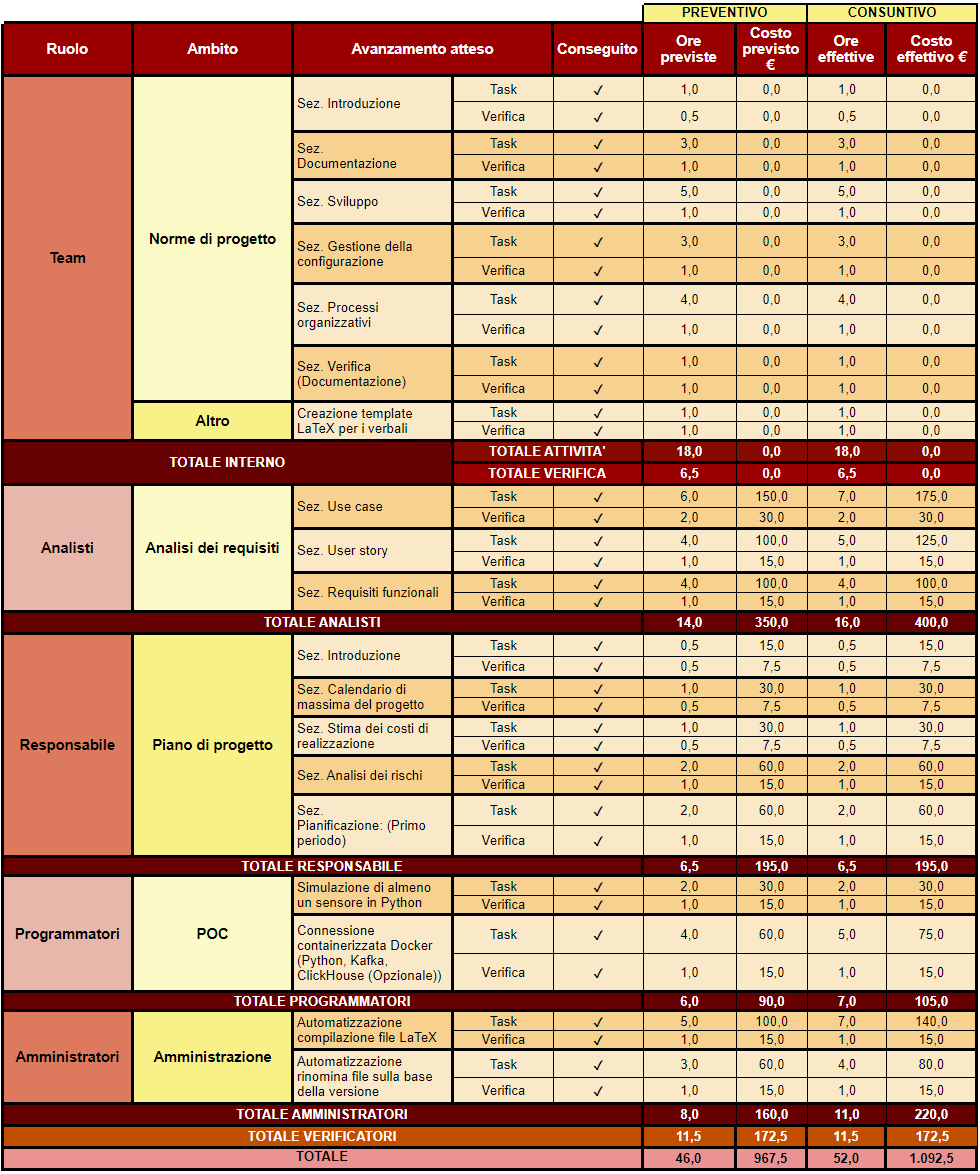
\includegraphics[height=0.9\textwidth]{../Images/periodo1.PNG}
    \caption{Primo periodo}
    \label{fig:Primo_periodo}
\end{figure}

Al termine del primo periodo, l'ammontare parziale totale del costo del progetto è \textbf{ 1317,50\euro\ } e sono state completate il \textbf{100\%} delle attività attese.
\href{https://github.com/orgs/ByteOps-swe/projects/3/views/1?sortedBy%5Bdirection%5D=asc&sortedBy%5BcolumnId%5D=64182560}{Vai al Diagramma di Gantt.}
\hspace{1pt}
  \begin{figure}[H]
    \centering
    \begin{minipage}[b]{0.45\textwidth}
        \centering
        \begin{tikzpicture}
            \pie[
                text=legend,
                color={blue!50, red!80}, 
                radius=2, 
                line width=0pt
            ]{10/Speso, 90/Rimanente}
        \end{tikzpicture}
        \caption{Grafico a torta del budget speso e rimanente preventivato - primo periodo}
        \label{fig:Budget_speso_1}
    \end{minipage}
    
    \vspace{1cm}

    \begin{minipage}[b]{0.70\textwidth}
        \centering
        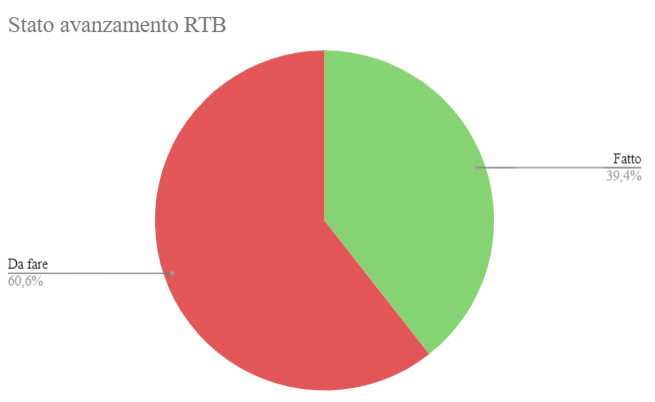
\includegraphics[width=0.7\textwidth]{../Images/avanzamento1Periodo.png}
        \caption{Avanzamento dei lavori RTB - primo periodo}
        \label{fig:Avanzamento_RTB_1}
    \end{minipage}
\end{figure}

\paragraph{Preventivo e consuntivo orario per membro}
Per le attività registrate nei costi, sono stati assegnati i seguenti ruoli: 

\begin{table}[H]
    \centering
    \begin{tabular}{|l|l|}
        \hline
        \textbf{Ruolo} & \textbf{Persona} \\
        \hline
        \hline
        Responsabile (Re) & F. Pozza \\
        \hline
        Amministratore (Am) & L. Skenderi \\
        \hline
        Analisti (An) & A. Barutta \\
        & R. Smanio \\
        \hline
        Verificatore (Ve) & E. Hysa \\
        \hline
        Programmatori (Pr) & N. Preto \\
        & D. Diotto \\
        \hline
        Progettista (Pt) & Nessuno \\
        \hline
    \end{tabular}
    \caption{Tabella dei Ruoli e delle Persone - primo periodo}
    \label{tab:Ruoli_persone_1}
    \end{table}

\paragraph*{Preventivo orario} \hspace{1pt}

\begin{figure}[H]
    \centering
    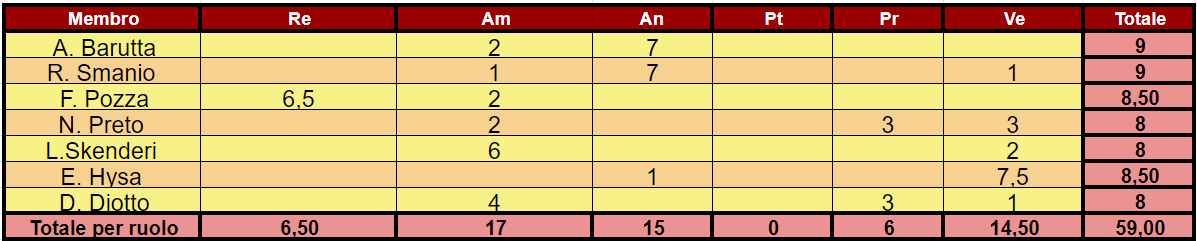
\includegraphics[width=0.9\textwidth]{../Images/preventivoOrario1Periodo.png}
    \caption{Preventivo orario per membro - primo periodo}
    \label{fig:Preventivo_orario_1}
\end{figure}

\begin{figure}[H]
    \centering
    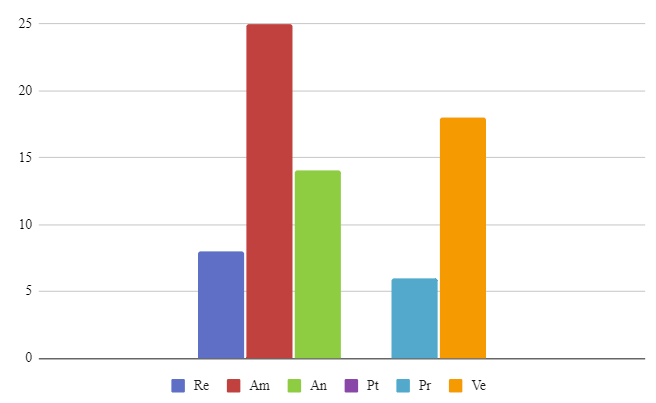
\includegraphics[width=0.6\textwidth]{../Images/preventivoDivisioneRuoli1Periodo.png}
    \caption{Istogramma preventivo della ripartizione oraria dei ruoli - primo periodo}
    \label{fig:Preventivo_ripartizione_oraria_1}
\end{figure}

\paragraph*{Consuntivo orario} \hspace{1pt}

\begin{figure}[H]
    \centering
    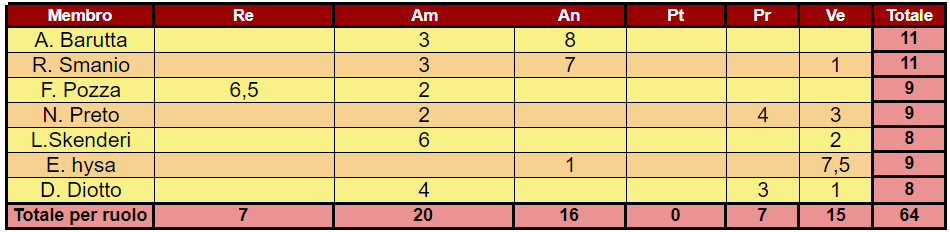
\includegraphics[width=0.9\textwidth]{../Images/consuntivoOrario1Periodo.png}
    \caption{Consuntivo orario per membro - primo periodo}
    \label{fig:Constuntivo_orario_1}
\end{figure}

\begin{figure}[H]
    \centering
    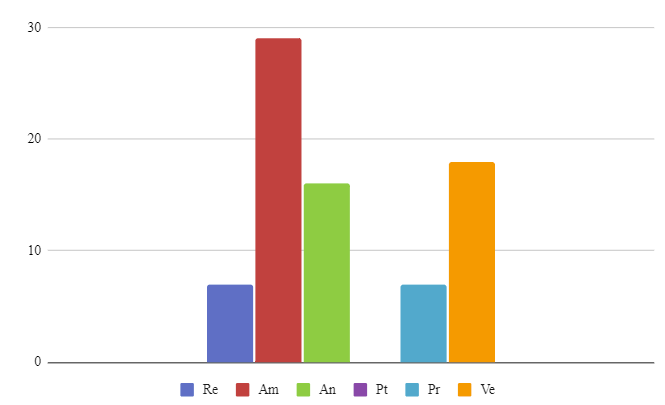
\includegraphics[width=0.6\textwidth]{../Images/consuntivoDivisioneRuoli1Periodo.png}
    \caption{Istogramma consuntivo della ripartizione oraria dei ruoli - primo periodo}
    \label{fig:Consuntivo_ripartizione_oraria_1}
\end{figure}

%________________________-SECONDO PERIODO-_____________________________

\subsubsection{Secondo periodo  24/11/2023 - 08/12/2023}
Durante il secondo periodo, il nostro team ha impegnato risorse per proseguire e completare parzialmente la definizione delle norme nel documento "Norme di progetto".

Nel corso del SAL con il proponente, è stato stabilito l'obiettivo di concludere entro la fine del secondo sprint la fase relativa al Proof of Concept (POC), focalizzata sull'integrazione dell'ultimo elemento nello stack tecnologico, "Grafana", e sulla visualizzazione di grafici delle misurazioni dei simulatori sviluppati.

È soddisfacente constatare che tutte le richieste del proponente sono state risolte entro i tempi concordati, portando così a termine lo sviluppo del POC.

Successivamente a un colloquio con il Prof. Cardin e al suo reindirizzamento sui casi d'uso, gli analisti hanno ridefinito parte di essi, causando un arretramento nel progresso verso la conclusione della RTB.

L'amministratore ha redatto il glossario di progetto e definito gli standard e le metriche di qualità di processo e prodotti nel documento "Piano di qualifica".

\paragraph{Rischi occorsi, impatto, mitigazione} 

Nel corso del secondo periodo, si sono presentate le seguenti problematiche:
\begin{itemize}
    \item \textbf{Assenza di uno dei membri per 4 giorni - \ref{sec:ImpPersonali}}
    \begin{itemize}
        \item \textbf{Esito mitigazione:} 
        L'azione di mitigazione adottata si è dimostrata efficace, senza suscitare proposte di modifiche.
        \item \textbf{Impatto:}
        Non sono emerse conseguenze significative; conformemente al processo di mitigazione, il responsabile ha ridistribuito i compiti del membro assente assegnandoli a ruoli con un carico lavorativo ridotto durante il periodo di assenza del membro.
        \end{itemize}
\end{itemize}

\newpage
\paragraph{Pianificazione attività divise per ruoli con consuntivo e preventivo orario e dei costi}\hspace{1pt}

\begin{figure}[H]
    \centering
    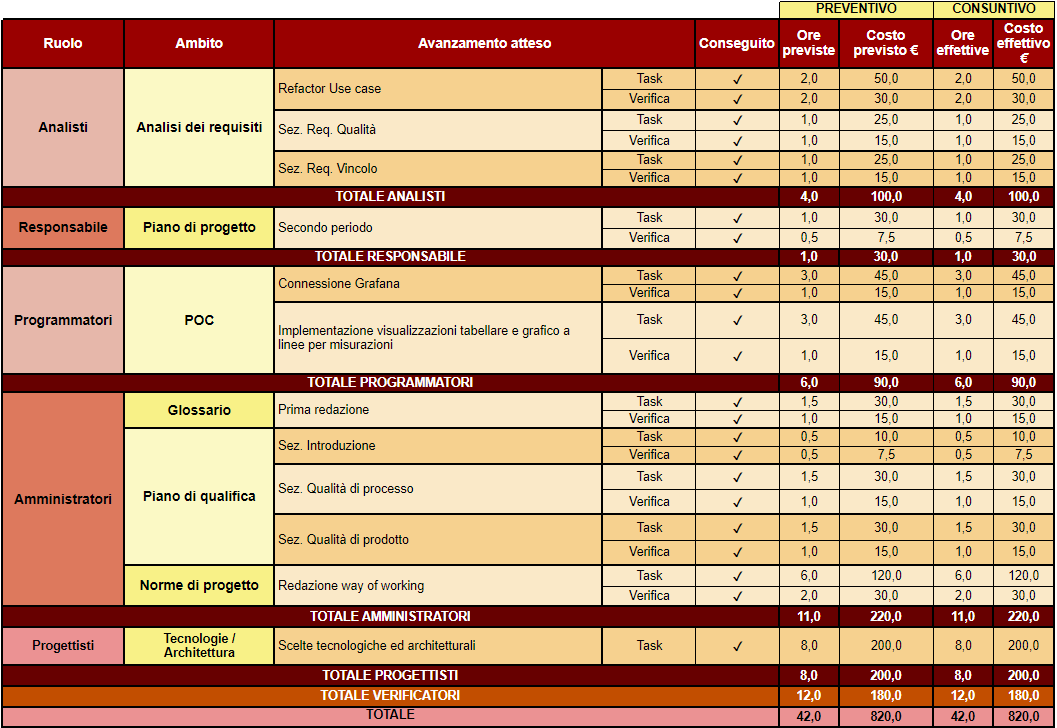
\includegraphics[width=\linewidth, height=0.9\textheight, keepaspectratio]{../Images/periodo2.PNG}
    \caption{Secondo periodo}
    \label{fig:Secondo_periodo}
\end{figure}

Al termine del secondo periodo, l'ammontare parziale totale del costo del progetto è \textbf{ 1937,50\euro\ } e sono state completate il \textbf{100\%} delle attività attese.
\href{https://github.com/orgs/ByteOps-swe/projects/3/views/1?sortedBy%5Bdirection%5D=asc&sortedBy%5BcolumnId%5D=64182560}{Vai al Diagramma di Gantt.}


\begin{figure}[H]
    \centering
    \begin{minipage}[b]{0.45\textwidth}
        \centering
        \begin{tikzpicture}
            \pie[
                text=legend,
                color={blue!50, red!80}, 
                radius=2, 
                line width=0pt
            ]{15/Speso, 85/Rimanente}
        \end{tikzpicture}
        \caption{Grafico a torta del budget speso e rimanente preventivato - secondo periodo}
        \label{fig:Budget_speso_2}
    \end{minipage}
    
    \vspace{1cm}

    \begin{minipage}[b]{0.70\textwidth}
        \centering
        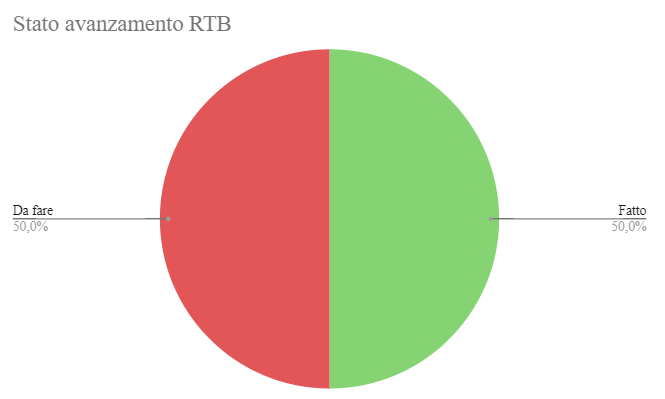
\includegraphics[width=0.7\textwidth]{../Images/avanzamento2Periodo.png}
        \caption{Avanzamento dei lavori RTB - secondo periodo}
        \label{fig:Avanzamento_RTB_2}
    \end{minipage}
\end{figure}

\paragraph{Preventivo e consuntivo orario per membro}
Per le attività registrate nei costi, sono stati assegnati i seguenti ruoli:

\begin{table}[H]
    \centering
    \begin{tabular}{|l|l|}
    \hline
    \textbf{Ruolo} & \textbf{Persona} \\
    \hline
    \hline
    Responsabile (Re) & L. Skenderi \\
    \hline
    Amministratore (Am) & A. Barutta \\
    \hline
    Analisti (An) & E. Hysa \\
     & R. Smanio \\
     \hline
    Verificatore (Ve) & D. Diotto \\
     & R. Smanio \\
     \hline
    Programmatori (Pr) & N. Preto \\
     & F. Pozza \\
     \hline
    Progettista (Pt) & Nessuno \\
    \hline
    \end{tabular}
    \caption{Tabella dei Ruoli e delle Persone - Secondo periodo}
    \label{tab:Ruoli_persone_2}
    \end{table}
    

\paragraph*{Preventivo orario} \hspace{1pt}

\begin{figure}[H]
    \centering
    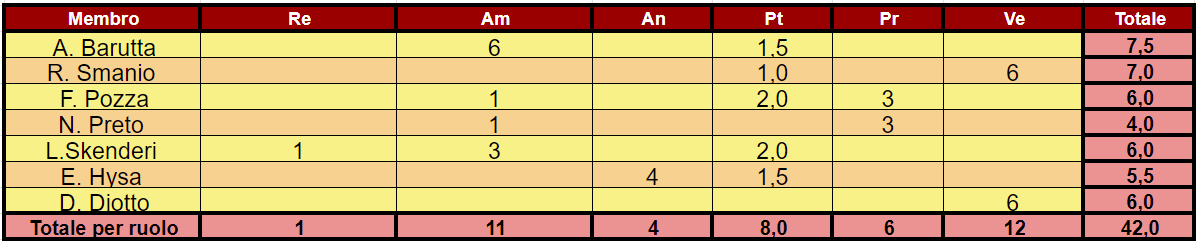
\includegraphics[width=0.9\textwidth]{../Images/preventivoOrario2Periodo.png}
    \caption{Preventivo orario per membro - secondo periodo}
    \label{fig:Preventivo_orario_2}
\end{figure}

\begin{figure}[H]
    \centering
    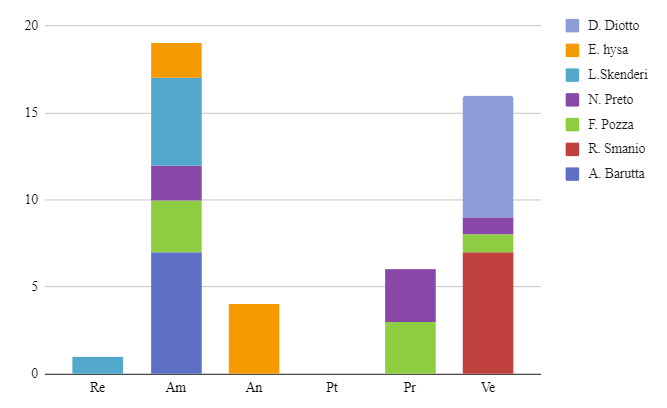
\includegraphics[width=0.6\textwidth]{../Images/preventivoDivisioneRuoli2Periodo.png}
    \caption{Istogramma preventivo della ripartizione oraria dei ruoli - secondo periodo}
    \label{fig:Preventivo_ripartizione_oraria_2}
\end{figure}

\paragraph*{Consuntivo orario } \hspace{1pt}

\begin{figure}[H]
    \centering
    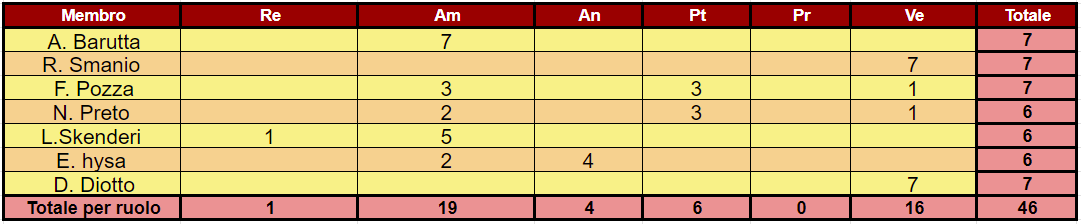
\includegraphics[width=0.9\textwidth]{../Images/consuntivoOrario2Periodo.png}
    \caption{Consuntivo orario per membro - secondo periodo}
    \label{fig:Constuntivo_orario_2}
\end{figure}

\begin{figure}[H]
    \centering
    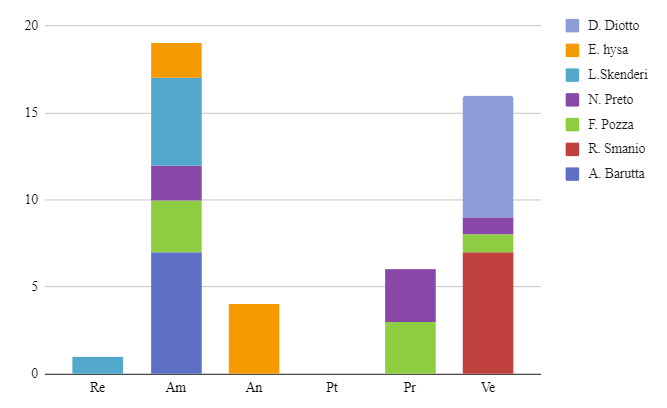
\includegraphics[width=0.6\textwidth]{../Images/consuntivoDivisioneRuoli2Periodo.png}
    \caption{Istogramma consuntivo della ripartizione oraria dei ruoli - secondo periodo}
    \label{fig:Consuntivo_ripartizione_oraria_2}
\end{figure}


%________________________-TERZO PERIODO-_____________________________


\subsubsection{Terzo periodo  08/12/2023 - 21/12/2023}
Nel corso del terzo periodo, il nostro team ha allocato risorse significative per condurre una revisione esaustiva del documento "Norme di progetto". L'amministratore si è concentrato sulla redazione del piano di qualifica, nonché sulla definizione e revisione delle metriche di qualità. Gli analisti hanno redatto e completato il refactor completo dell'Analisi dei requisiti, includendo la conclusione dei casi d'uso, dei requisiti funzionali, dei requisiti di vincolo, dei requisiti di qualità e del tracciamento. I programmatori hanno dedicato un impegno considerevole alla risoluzione di bug nel Proof of Concept (PoC) e alla creazione di una versione stabile destinata alla presentazione durante la revisione RTB.

\paragraph{Rischi occorsi, impatto, mitigazione} 

Nel corso del terzo periodo non si sono presentate problematiche.

\newpage
\paragraph{Pianificazione attività divise per ruoli con consuntivo e preventivo orario e dei costi}\hspace{1pt}

\begin{figure}[H]
    \centering
    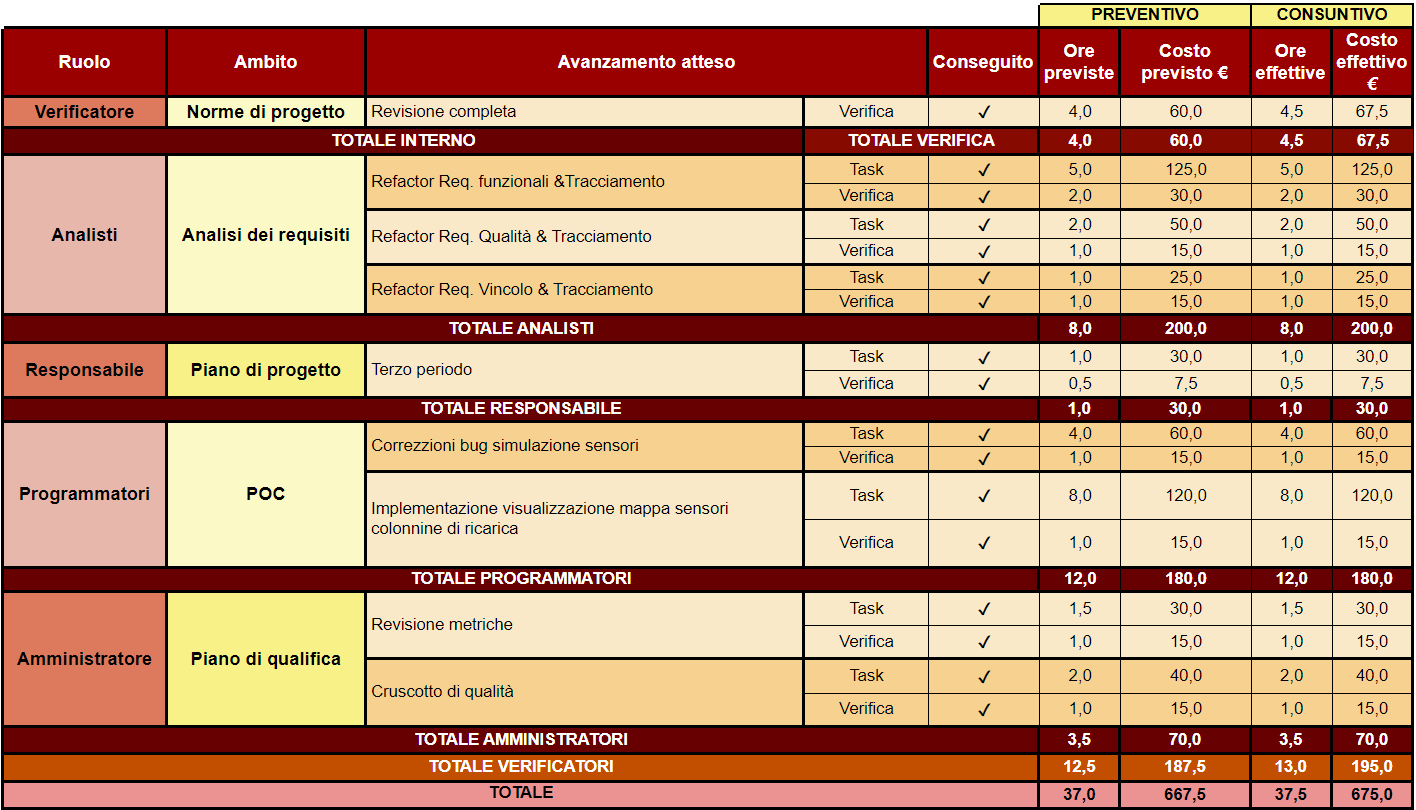
\includegraphics[width=\linewidth, height=0.9\textheight, keepaspectratio]{../Images/periodo3.PNG}
    \caption{Terzo periodo}
    \label{fig:Terzo_periodo}
\end{figure}


Al termine del terzo periodo, l'ammontare parziale totale del costo del progetto è \textbf{ 2612,5\euro\ } e sono state completate il \textbf{100\%} delle attività attese.
\href{https://github.com/orgs/ByteOps-swe/projects/3/views/1?sortedBy%5Bdirection%5D=asc&sortedBy%5BcolumnId%5D=64182560}{Vai al Diagramma di Gantt.}\hspace{1pt}


\begin{figure}[H]
    \centering
    \begin{minipage}[b]{0.45\textwidth}
        \centering
        \begin{tikzpicture}
            \pie[
                text=legend,
                color={blue!50, red!80}, 
                radius=2, 
                line width=0pt
            ]{21/Speso, 79/Rimanente}
        \end{tikzpicture}
        \caption{Grafico a torta del budget speso e rimanente preventivato - terzo periodo}
        \label{fig:Budget_speso_3}
    \end{minipage}
    
    \vspace{1cm}

    \begin{minipage}[b]{0.70\textwidth}
        \centering
        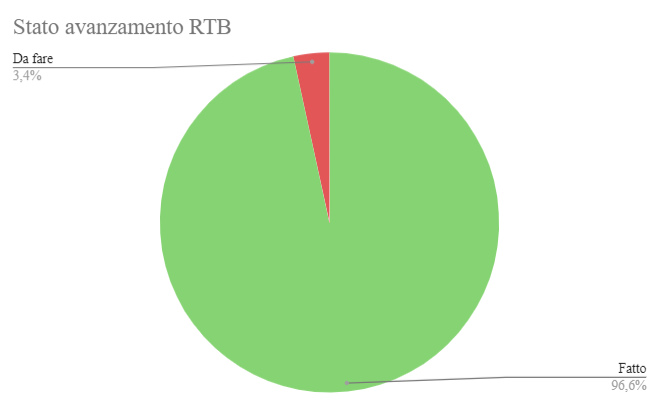
\includegraphics[width=0.7\textwidth]{../Images/avanzamento3Periodo.png}
        \caption{Avanzamento dei lavori RTB - terzo periodo}
        \label{fig:Avanzamento_RTB_3}
    \end{minipage}
\end{figure}

\paragraph{Preventivo e consuntivo orario per membro} \hspace{1pt}
Per le attività registrate nei costi, sono stati assegnati i seguenti ruoli:  

\begin{table}[H]
    \centering
    \begin{tabular}{|l|l|}
    \hline
    \textbf{Ruolo} & \textbf{Persona} \\
    \hline
    \hline
    Responsabile (Re) & R. Smanio \\
    \hline
    Amministratore (Am) & D. Diotto \\
    \hline
    Analisti (An) & L. Skenderi \\
    \hline
    Verificatore (Ve) & N. Preto \\
     & A. Barutta \\
     \hline
    Programmatori (Pr) & E. Hysa \\
     & F. Pozza \\
     \hline
    Progettista (Pt) & Nessuno \\
    \hline
    \end{tabular}
    \caption{Tabella dei Ruoli e delle Persone - Terzo periodo}
    \label{tab:Ruoli_persone_3}
    \end{table}
    

\paragraph*{Preventivo orario} \hspace{1pt}

\begin{figure}[H]
    \centering
    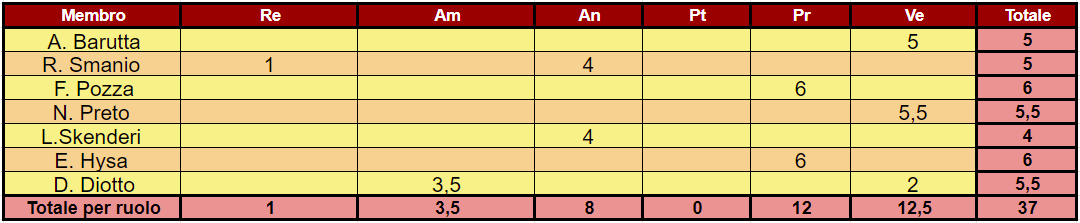
\includegraphics[width=0.9\textwidth]{../Images/preventivoOrario3Periodo.png}
    \caption{Preventivo orario per membro - terzo periodo}
    \label{fig:Preventivo_orario_3}
\end{figure}

\begin{figure}[H]
    \centering
    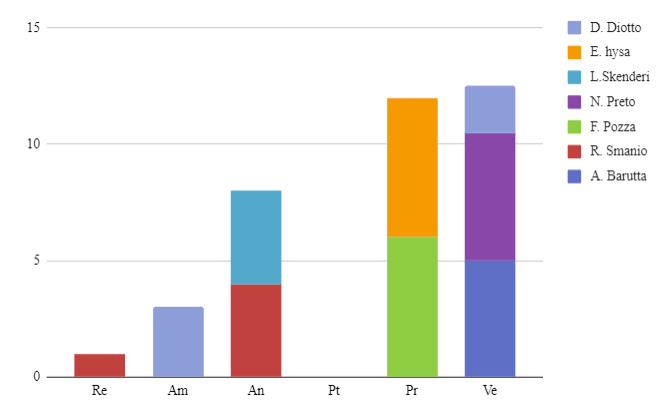
\includegraphics[width=0.6\textwidth]{../Images/preventivoDivisioneRuoli3Periodo.png}
    \caption{Istogramma preventivo della ripartizione oraria dei ruoli - terzo periodo}
    \label{fig:Preventivo_ripartizione_oraria_3}
\end{figure}

\paragraph*{Consuntivo orario } \hspace{1pt}

\begin{figure}[H]
    \centering
    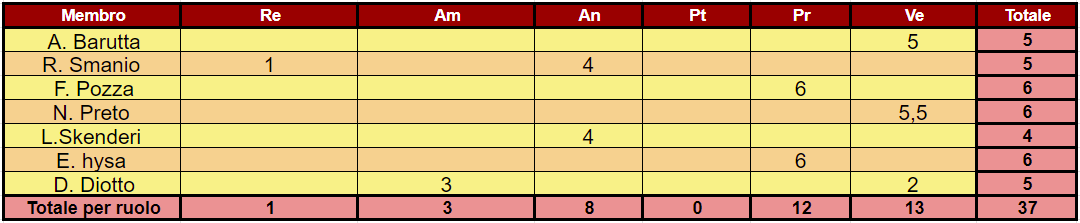
\includegraphics[width=0.9\textwidth]{../Images/consuntivoOrario3Periodo.png}
    \caption{Consuntivo orario per membro - terzo periodo}
    \label{fig:Constuntivo_orario_3}
\end{figure}

\begin{figure}[H]
    \centering
    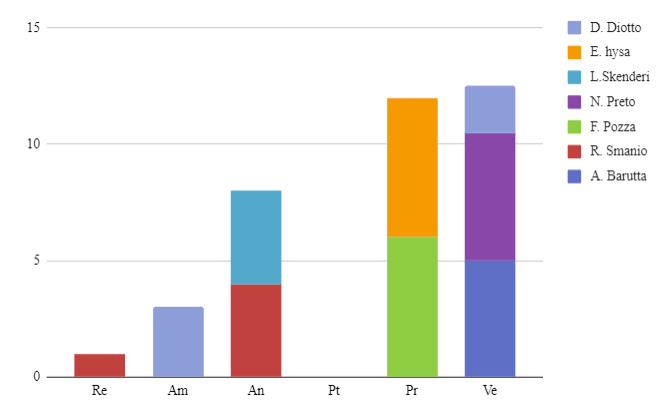
\includegraphics[width=0.6\textwidth]{../Images/consuntivoDivisioneRuoli3Periodo.png}
    \caption{Istogramma consuntivo della ripartizione oraria dei ruoli - terzo periodo}
    \label{fig:Consuntivo_ripartizione_oraria_3}
\end{figure}


%________________________-QUARTO PERIODO-_____________________________


\subsubsection{Quarto periodo  21/12/2023 - 07/12/2024}

Il quarto periodo è stato principalmente focalizzato sul potenziamento e perfezionamento dell'analisi dei requisiti. Ciò ha comportato un miglioramento delle descrizioni dei casi d'uso, delle use stories, dei requisiti e del tracciamento. Le attività di programmazione si sono svolte mirando a garantire solidità ed efficienza del prodotto (PoC) in vista della revisione RTB. Inoltre, è stata creata una pagina su GitHub io per consentire una navigazione chiara e rapida della repository del progetto.

Durante questo periodo, sono state instanziate rilevanti risorse per condurre attività di verifica su tutti i configuration item prodotti nel corso dei quattro periodi.

\paragraph{Rischi occorsi, impatto, mitigazione} 
Nel corso del quarto periodo, si sono presentate le seguenti problematiche:
\begin{itemize}
    \item \textbf{Rallentamento del progetto dovuto all’armonizzazione delle attività personali - \ref{sec:ImpPersonali}}
    \begin{itemize}
        \item \textbf{Esito mitigazione:} 
        Il responsabile in accordo con la proponente ha prudentemente vincolato il numero di attività avviate durante questo periodo, estendendo contemporaneamente i tempi, al fine di assicurare il completo svolgimento di tutte le attività pianificate.
        \item \textbf{Impatto:}
        In vista dell'imminente avvio della sessione invernale, si è verificato un rallentamento delle attività di progetto a causa degli impegni accademici dei membri del team.
        \end{itemize}
\end{itemize}

\newpage
\paragraph{Pianificazione attività divise per ruoli con consuntivo e preventivo orario e dei costi}\hspace{1pt}

\begin{figure}[H]
    \centering
    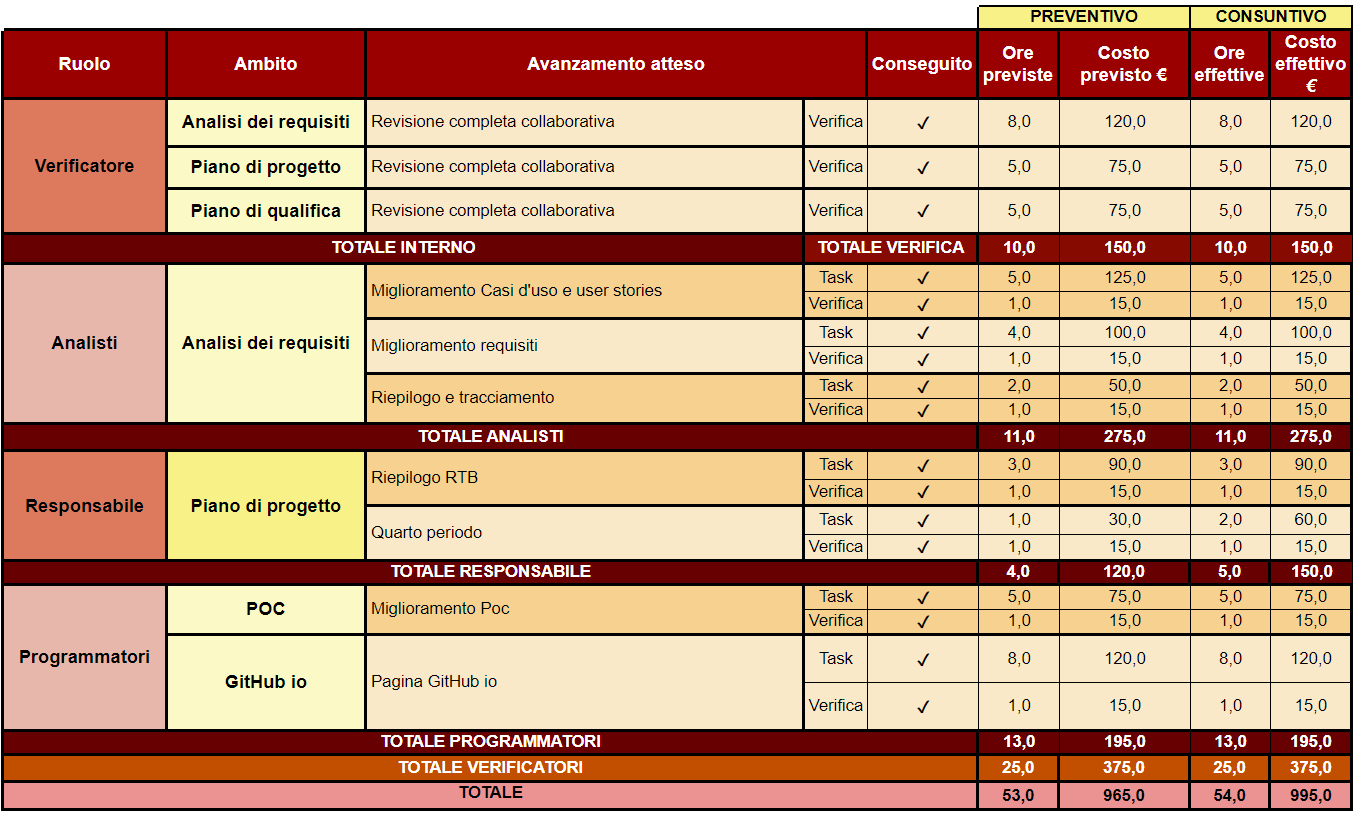
\includegraphics[width=\linewidth, height=0.9\textheight, keepaspectratio]{../Images/periodo4.PNG}
    \caption{Quarto periodo}
    \label{fig:Quarto_periodo}
\end{figure}


Al termine del terzo periodo, l'ammontare parziale totale del costo del progetto è \textbf{ 3607,5\euro\ } e sono state completate il \textbf{100\%} delle attività attese.
\href{https://github.com/orgs/ByteOps-swe/projects/3/views/1?sortedBy%5Bdirection%5D=asc&sortedBy%5BcolumnId%5D=64182560}{Vai al Diagramma di Gantt.}\hspace{1pt}


\begin{figure}[H]
    \centering
    \begin{minipage}[b]{0.45\textwidth}
        \centering
        \begin{tikzpicture}
            \pie[
                text=legend,
                color={blue!50, red!80}, 
                radius=2, 
                line width=0pt
            ]{29/Speso, 71/Rimanente}
        \end{tikzpicture}
        \caption{Grafico a torta del budget speso e rimanente preventivato - quarto periodo}
        \label{fig:Budget_speso_4}
    \end{minipage}
    
    \vspace{1cm}

    \begin{minipage}[b]{0.70\textwidth}
        \centering
        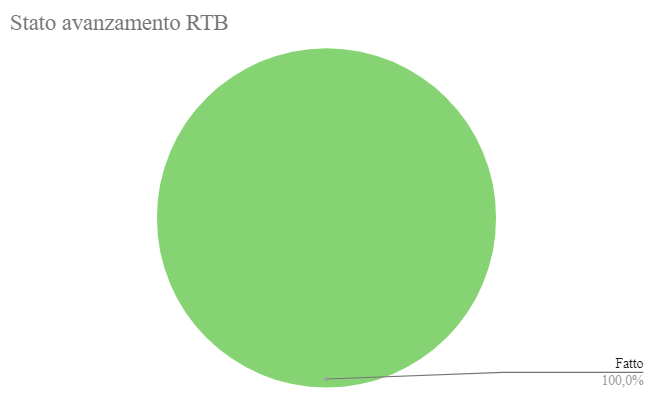
\includegraphics[width=0.7\textwidth]{../Images/avanzamento4Periodo.png}
        \caption{Avanzamento dei lavori RTB - quarto periodo}
        \label{fig:Avanzamento_RTB_4}
    \end{minipage}
\end{figure}

\paragraph{Preventivo e consuntivo orario per membro} \hspace{1pt}
Per le attività registrate nei costi, sono stati assegnati i seguenti ruoli: (durante tale periodo, alcuni membri del team hanno assunto più responsabilità, conformemente a quanto concordato sin dall'inizio del periodo).

\begin{table}[H]
    \centering
    \begin{tabular}{|l|l|}
    \hline
    \textbf{Ruolo} & \textbf{Persona} \\
    \hline
    \hline
    Responsabile (Re) & N. Preto \\
    \hline
    Amministratore (Am) & E. Hysa \\
    \hline
    Analisti (An)   & F. Pozza \\
                    & D. Diotto \\
    \hline
    Verificatore (Ve)   & L. Skenderi \\
                        & N. Preto \\
                        & E. Hysa \\
     \hline
    Programmatori (Pr)  & A. Barutta \\
                        & R. Smanio \\
    \hline
    Progettista (Pt) & Nessuno \\
    \hline
    \end{tabular}
    \caption{Tabella dei Ruoli e delle Persone - Quarto periodo}
    \label{tab:Ruoli_persone_4}
    \end{table}
    

\paragraph*{Preventivo orario} \hspace{1pt}

\begin{figure}[H]
    \centering
    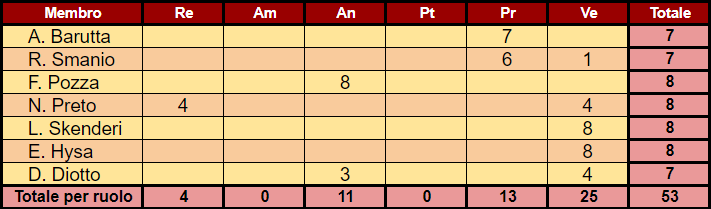
\includegraphics[width=0.9\textwidth]{../Images/preventivoOrario4Periodo.png}
    \caption{Preventivo orario per membro - quarto periodo}
    \label{fig:Preventivo_orario_4}
\end{figure}

\begin{figure}[H]
    \centering
    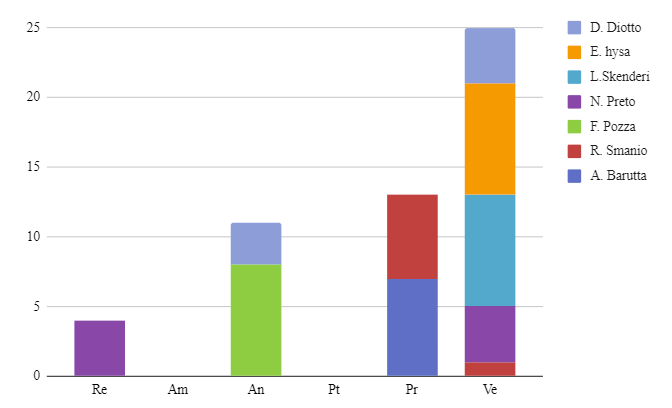
\includegraphics[width=0.6\textwidth]{../Images/preventivoDivisioneRuoli4Periodo.png}
    \caption{Istogramma preventivo della ripartizione oraria dei ruoli - quarto periodo}
    \label{fig:Preventivo_ripartizione_oraria_4}
\end{figure}

\paragraph*{Consuntivo orario } \hspace{1pt}

\begin{figure}[H]
    \centering
    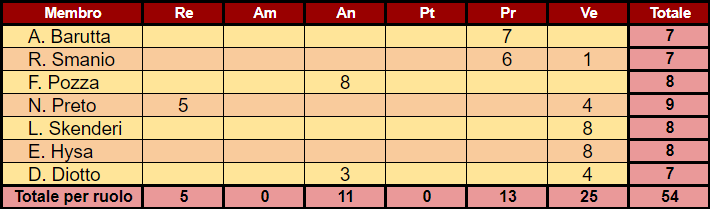
\includegraphics[width=0.9\textwidth]{../Images/consuntivoOrario4Periodo.png}
    \caption{Consuntivo orario per membro - quarto periodo}
    \label{fig:Constuntivo_orario_4}
\end{figure}

\begin{figure}[H]
    \centering
    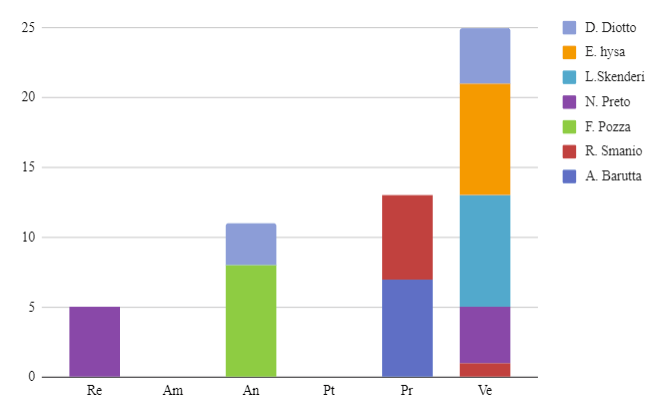
\includegraphics[width=0.6\textwidth]{../Images/consuntivoDivisioneRuoli4Periodo.png}
    \caption{Istogramma consuntivo della ripartizione oraria dei ruoli - quarto periodo}
    \label{fig:Consuntivo_ripartizione_oraria_4}
\end{figure}

%________________________-QUINTO PERIODO-_____________________________


\subsubsection{Quinto periodo  07/01/2024 - 15/01/2024}
In seguito al completamento delle attività concernenti la baseline RTB, il team ha impiegato risorse per sviluppare le presentazioni correlate, sia per la parte relativa al professor Cardin che per quella relativa al professor Vardanega.
È importante notare che il compito eseguito dagli amministratori e le risorse ad esso allocate non sono state incluse nel calcolo dei costi. 
In aggiunta, sono stati apportati lievi ritocchi di formalizzazione ai documenti.

\paragraph{Gestione dei rischi} 
Nel corso del quinto periodo, sono previste e sono occorse le seguenti problematiche:
\begin{itemize}
    \item \textbf{Rallentamento del progetto dovuto all’armonizzazione delle attività personali - \ref{sec:ImpPersonali}}
    \begin{itemize}
        \item \textbf{Esito mitigazione:} 
        In seguito a una concorde decisione tra il responsabile e la proponente, è stato prudentemente limitato il numero di attività avviate durante questo periodo. Ulteriormente, considerando l'approssimarsi della sessione invernale di esami, si è provveduto a ridurre l'ampiezza temporale a una settimana.
        \item \textbf{Impatto:}
        L'avanzamento procede a ritmo più lento, tuttavia tale andamento è conforme a quanto preventivato durante la fase di pianificazione.
    \end{itemize}
\end{itemize}
\newpage
\paragraph{Pianificazione attività divise per ruoli con consuntivo e preventivo orario e dei costi}\hspace{1pt}

\begin{figure}[H]
    \centering
    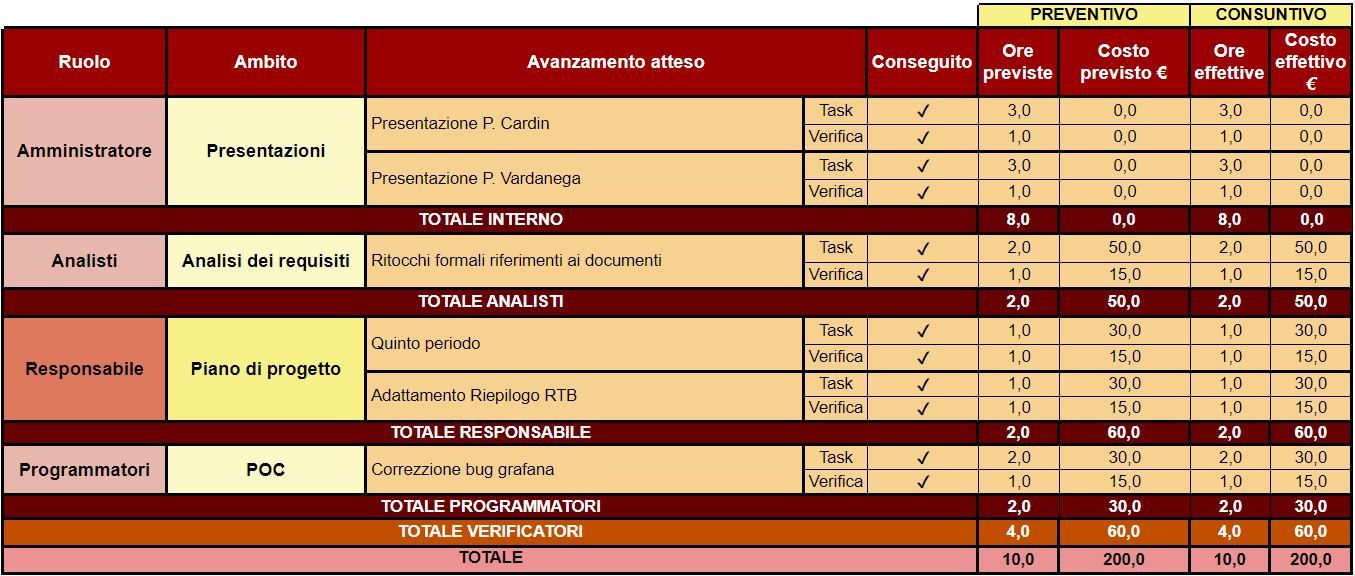
\includegraphics[width=\linewidth, height=0.9\textheight, keepaspectratio]{../Images/periodo5.PNG}
    \caption{quinto periodo}
    \label{fig:Quarto_periodo}
\end{figure}

Al termine del secondo periodo, l'ammontare parziale totale del costo del progetto è \textbf{ 3807,50\euro\ } e sono state completate il \textbf{100\%} delle attività attese.


\begin{figure}[H]
    \centering
    \begin{minipage}[b]{0.45\textwidth}
        \centering
        \begin{tikzpicture}
            \pie[
                text=legend,
                color={blue!50, red!80}, 
                radius=2, 
                line width=0pt
            ]{30/Speso, 70/Rimanente}
        \end{tikzpicture}
        \caption{Grafico a torta del budget speso e rimanente preventivato - quinto periodo}
        \label{fig:Budget_speso_4}
    \end{minipage}
    \vspace{1cm}
\end{figure}

\paragraph{Preventivo e consuntivo orario per membro} \hspace{1pt}
Per le attività registrate nei costi, sono stati assegnati i seguenti ruoli:

\begin{table}[H]
    \centering
    \begin{tabular}{|l|l|}
    \hline
    \textbf{Ruolo} & \textbf{Persona} \\
    \hline
    \hline
    Responsabile (Re) & D. Diotto \\
    \hline
    Amministratore (Am) & A.Barutta  \\
    & R. Smanio \\
    \hline
    Analisti (An)   & E. Hysa \\
    & N. Preto \\
    \hline
    Verificatore (Ve)   & F. Pozza \\
    & L. Skenderi\\
     \hline
    Programmatori (Pr)  & L. Skenderi \\    
    \hline
    Progettista (Pt) & Nessuno \\
    \hline
    \end{tabular}
    \caption{Tabella dei Ruoli e delle Persone - Quinto periodo}
    \label{tab:Ruoli_persone_4}
    \end{table}
    

\paragraph*{Preventivo orario} \hspace{1pt}

\begin{figure}[H]
    \centering
    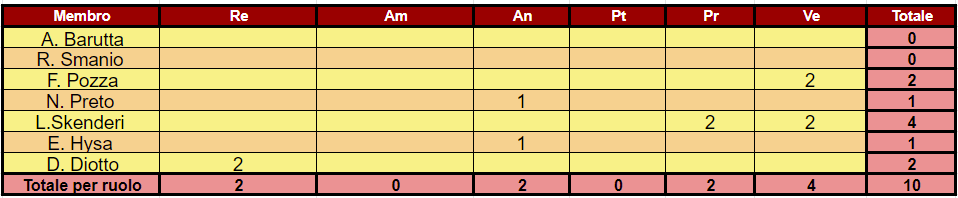
\includegraphics[width=0.9\textwidth]{../Images/preventivoOrario5Periodo.png}
    \caption{Preventivo orario per membro - quinto periodo}
    \label{fig:Preventivo_orario_4}
\end{figure}

\begin{figure}[H]
    \centering
    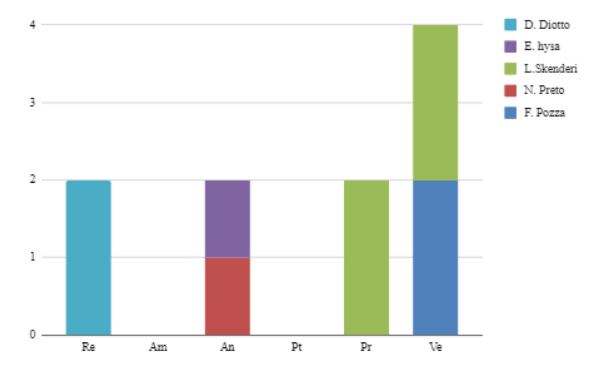
\includegraphics[width=0.6\textwidth]{../Images/preventivoDivisioneRuoli5Periodo.png}
    \caption{Istogramma preventivo della ripartizione oraria dei ruoli - quinto periodo}
    \label{fig:Preventivo_ripartizione_oraria_4}
\end{figure}

\paragraph*{Consuntivo orario } \hspace{1pt}

\begin{figure}[H]
    \centering
    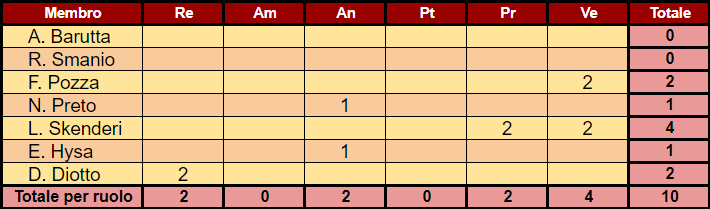
\includegraphics[width=0.9\textwidth]{../Images/consuntivoOrario5Periodo.png}
    \caption{Consuntivo orario per membro - quinto periodo}
    \label{fig:Constuntivo_orario_4}
\end{figure}

\begin{figure}[H]
    \centering
    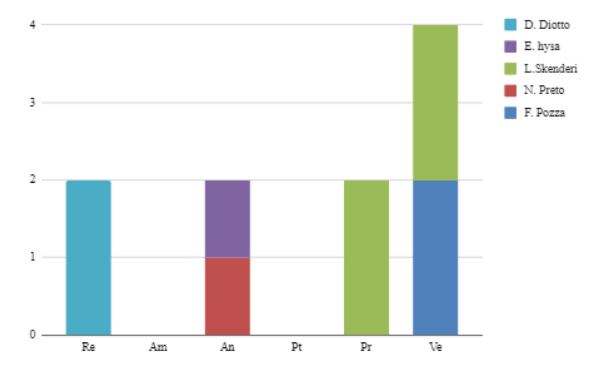
\includegraphics[width=0.6\textwidth]{../Images/consuntivoDivisioneRuoli5Periodo.png}
    \caption{Istogramma consuntivo della ripartizione oraria dei ruoli - quinto periodo}
    \label{fig:Consuntivo_ripartizione_oraria_4}
\end{figure}
%________________________-Sesto PERIODO-_____________________________


\subsubsection{Sesto periodo  15/01/2024 - 01/02/2024}
Per quanto attiene all'organizzazione di questo periodo, in considerazione della sovrapposizione con l'inizio della sessione di esami, il gruppo ha unanimemente raggiunto un accordo. Oltre a dedicarsi alla preparazione per i colloqui della RTB, abbiamo deliberato di focalizzarci principalmente sullo studio individuale necessario per affrontare la sessione stessa, evitando ulteriori avanzamenti nel progetto.

In questo periodo quindi, ci dedicheremo esclusivamente alla rifinitura dei dettagli concernenti le presentazioni destinate al Prof Cardin e al Prof. Vardanega.

\paragraph{Gestione dei rischi} 
Nel corso del sesto periodo,sono previste e occorse le seguenti problematiche:
\begin{itemize}
    \item \textbf{Rallentamento del progetto dovuto all’armonizzazione delle attività personali - \ref{sec:ImpPersonali}}
    \begin{itemize}
        \item \textbf{Impatto:}
       L'avanzamento del progetto è nullo in questo periodo ma ciò è conforme a quanto preventivato
    \end{itemize}
\end{itemize}
\newpage
\paragraph{Pianificazione attività, preventivo e consuntivo}\hspace{1pt}
Non è previsto e pianificato avanzamento effettivo all’interno di questo periodo, se non per ciò che riguarda
le presentazioni relative alla RTB.
Di conseguenza non vengono riportati preventivi e consuntivi di periodo.
